\chapter{Geometry}

\index{geometry}

In geometric problems, it is often challenging
to find a way to approach the problem so that
the solution to the problem can be conveniently implemented
and the number of special cases is small.

As an example, consider a problem where
we are given the vertices of a quadrilateral
(a polygon that has four vertices),
and our task is to calculate its area.
For example, a possible input for the problem is as follows:

\begin{center}
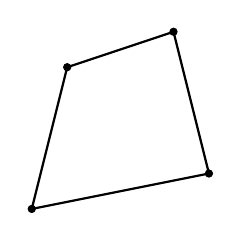
\begin{tikzpicture}[scale=0.45]

\draw[fill] (6,2) circle [radius=0.1];
\draw[fill] (5,6) circle [radius=0.1];
\draw[fill] (2,5) circle [radius=0.1];
\draw[fill] (1,1) circle [radius=0.1];
\draw[thick] (6,2) -- (5,6) -- (2,5) -- (1,1) -- (6,2);
\end{tikzpicture}
\end{center}
One way to approach the problem is to divide
the quadrilateral into two triangles by a straight
line between two opposite vertices:
\begin{center}
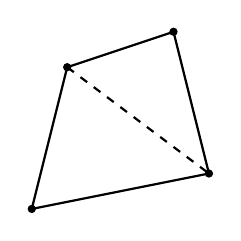
\begin{tikzpicture}[scale=0.45]

\draw[fill] (6,2) circle [radius=0.1];
\draw[fill] (5,6) circle [radius=0.1];
\draw[fill] (2,5) circle [radius=0.1];
\draw[fill] (1,1) circle [radius=0.1];

\draw[thick] (6,2) -- (5,6) -- (2,5) -- (1,1) -- (6,2);
\draw[dashed,thick] (2,5) -- (6,2);
\end{tikzpicture}
\end{center}
After this, it suffices to sum the areas
of the triangles.
The area of a triangle can be calculated,
for example, using \key{Heron's formula}
%\footnote{Heron of Alexandria (c. 10--70) was a Greek mathematician.}
\[ \sqrt{s (s-a) (s-b) (s-c)},\]
where $a$, $b$ and $c$ are the lengths
of the triangle's sides and
$s=(a+b+c)/2$.
\index{Heron's formula}

This is a possible way to solve the problem,
but there is one pitfall:
how to divide the quadrilateral into triangles?
It turns out that sometimes we cannot just pick
two arbitrary opposite vertices.
For example, in the following situation,
the division line is outside the quadrilateral:
\begin{center}
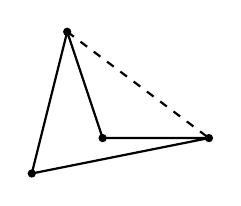
\begin{tikzpicture}[scale=0.45]

\draw[fill] (6,2) circle [radius=0.1];
\draw[fill] (3,2) circle [radius=0.1];
\draw[fill] (2,5) circle [radius=0.1];
\draw[fill] (1,1) circle [radius=0.1];
\draw[thick] (6,2) -- (3,2) -- (2,5) -- (1,1) -- (6,2);

\draw[dashed,thick] (2,5) -- (6,2);
\end{tikzpicture}
\end{center}
However, another way to draw the line works:
\begin{center}
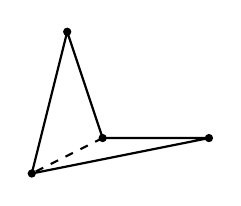
\begin{tikzpicture}[scale=0.45]

\draw[fill] (6,2) circle [radius=0.1];
\draw[fill] (3,2) circle [radius=0.1];
\draw[fill] (2,5) circle [radius=0.1];
\draw[fill] (1,1) circle [radius=0.1];
\draw[thick] (6,2) -- (3,2) -- (2,5) -- (1,1) -- (6,2);

\draw[dashed,thick] (3,2) -- (1,1);
\end{tikzpicture}
\end{center}
It is clear for a human which of the lines is the correct
choice, but the situation is difficult for a computer.
                           
However, it turns out that we can solve the problem using
another method that is much easier to implement
and does not involve any special cases.
Namely, there is a general formula
\[x_1y_2-x_2y_1+x_2y_3-x_3y_2+x_3y_4-x_4y_3+x_4y_1-x_1y_4,\]
that calculates the area of a quadrilateral
whose vertices are
$(x_1,y_1)$,
$(x_2,y_2)$,
$(x_3,y_3)$ and
$(x_4,y_4)$.
This formula is easy to implement, there are no special
cases, and it turns out that we can even generalize the formula
to \emph{all} polygons.

\section{Complex numbers}

\index{complex number}
\index{point}
\index{vector}

A \key{complex number} is a number of the form $x+y i$,
where $i = \sqrt{-1}$ is the \key{imaginary unit}.
A geometric interpretation of a complex number is
that it represents a two-dimensional point $(x,y)$
or a vector from the origin to a point $(x,y)$.

For example, $4+2i$ corresponds to the
following point and vector:

\begin{center}
\begin{tikzpicture}[scale=0.45]

\draw[->,thick] (-5,0)--(5,0);
\draw[->,thick] (0,-5)--(0,5);

\draw[fill] (4,2) circle [radius=0.1];
\draw[->,thick] (0,0)--(4-0.1,2-0.1);

\node at (4,2.8) {$(4,2)$};
\end{tikzpicture}
\end{center}

\index{complex@\texttt{complex}}

The complex number class \texttt{complex} in C++ is
useful when solving geometric problems.
Using the class we can represent points and vectors
as complex numbers, and the class also contains tools
that are useful in geometry.

In the following code, \texttt{C} is the type of
a coordinate and \texttt{P} is the type of a point or vector.
In addition, the code defines the macros \texttt{X} and \texttt{Y}
that can be used to refer to x and y coordinates.

\begin{lstlisting}
typedef long long C;
typedef complex<C> P;
#define X real()
#define Y imag()
\end{lstlisting}

For example, the following code defines a point $p=(4,2)$
and prints its x and y coordinates:

\begin{lstlisting}
P p = {4,2};
cout << p.X << " " << p.Y << "\n"; // 4 2
\end{lstlisting}

The following code defines vectors $v=(3,1)$ and $u=(2,2)$,
and after that calculates the sum $s=v+u$.

\begin{lstlisting}
P v = {3,1};
P u = {2,2};
P s = v+u;
cout << s.X << " " << s.Y << "\n"; // 5 3
\end{lstlisting}

An appropriate coordinate type is
\texttt{long long} (integer) or \texttt{long double}
(real number), depending on the situation.
Integers should be used whenever possible,
because calculations with integers are exact.
If real numbers are needed,
precision errors should be taken into account
when comparing them.
A safe way to check if numbers $a$ and $b$ are equal
is to compare them using $|a-b|<\epsilon$,
where $\epsilon$ is a small number (for example, $\epsilon=10^{-9}$).

\subsubsection*{Functions}

In the following examples, the coordinate type is
\texttt{long double}.

The function \texttt{abs(v)} calculates the length
$|v|$ of a vector $v=(x,y)$
using the formula $\sqrt{x^2+y^2}$.
The function can also be used for
calculating the distance between points
$(x_1,y_1)$ and $(x_2,y_2)$,
because that distance equals the length
of the vector $(x_2-x_1,y_2-y_1)$.

The following code calculates the distance
between points $(4,2)$ and $(3,-1)$:
\begin{lstlisting}
P a = {4,2};
P b = {3,-1};
cout << abs(b-a) << "\n"; // 3.60555
\end{lstlisting}

The function \texttt{arg(v)} calculates the
angle of a vector $v=(x,y)$ with respect to the x axis.
The function gives the angle in radians,
where $r$ radians equals $180 r/\pi$ degrees.
The angle of a vector that points to the right is 0,
and angles decrease clockwise and increase
counterclockwise.

The function \texttt{polar(s,a)} constructs a vector
whose length is $s$ and that points to an angle $a$.
In addition, a vector can be rotated by an angle $a$
by multiplying it by a vector with length 1 and angle $a$.

The following code calculates the angle of
the vector $(4,2)$, rotates it $1/2$ radians
counterclockwise, and then calculates the angle again:

\begin{lstlisting}
P v = {4,2};
cout << arg(v) << "\n"; // 0.463648
v *= polar(1.0,0.5);
cout << arg(v) << "\n"; // 0.963648
\end{lstlisting}

\section{Points and lines}

\index{cross product}

The \key{cross product} $a \times b$ of vectors
$a=(x_1,y_1)$ and $b=(x_2,y_2)$ equals $x_1 y_2 - x_2 y_1$.
The cross product tells us whether $b$
turns left (positive value), does not turn (zero)
or turns right (negative value)
when it is placed directly after $a$.

The following picture illustrates the above cases:
\begin{center}
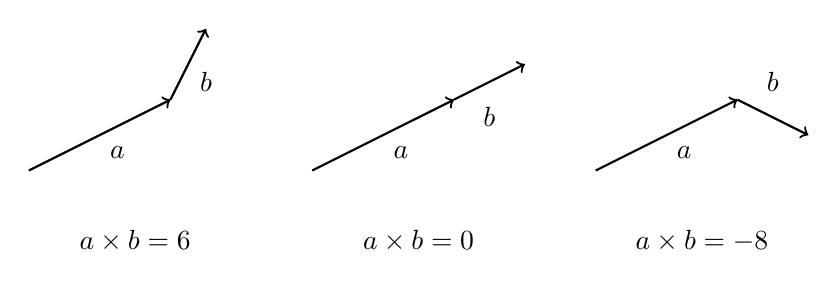
\begin{tikzpicture}[scale=0.45]

\draw[->,thick] (0,0)--(4,2);
\draw[->,thick] (4,2)--(4+1,2+2);

\node at (2.5,0.5) {$a$};
\node at (5,2.5) {$b$};

\node at (3,-2) {$a \times b = 6$};

\draw[->,thick] (8+0,0)--(8+4,2);
\draw[->,thick] (8+4,2)--(8+4+2,2+1);

\node at (8+2.5,0.5) {$a$};
\node at (8+5,1.5) {$b$};

\node at (8+3,-2) {$a \times b = 0$};

\draw[->,thick] (16+0,0)--(16+4,2);
\draw[->,thick] (16+4,2)--(16+4+2,2-1);

\node at (16+2.5,0.5) {$a$};
\node at (16+5,2.5) {$b$};

\node at (16+3,-2) {$a \times b = -8$};
\end{tikzpicture}
\end{center}

\noindent
For example, in the first picture
$a=(4,2)$ and $b=(1,2)$.
The following code calculates the cross product
using the class \texttt{complex}:

\begin{lstlisting}
P a = {4,2};
P b = {1,2};
C r = (conj(a)*b).Y; // 6
\end{lstlisting}

The above code works, because
the function \texttt{conj} negates the y coordinate
of a vector,
and when the vectors $(x_1,-y_1)$ and $(x_2,y_2)$
are multiplied together, the y coordinate
of the result is $x_1 y_2 - x_2 y_1$.

\subsubsection{Point location}

Cross products can be used for testing
whether a point is located on the left or right
side of a line.
Assume that the line goes through points
$s_1$ and $s_2$, we are looking from $s_1$
to $s_2$ and the point is $p$.

For example, in the following picture,
$p$ is on the left side of the line:
\begin{center}
\begin{tikzpicture}[scale=0.45]
\draw[dashed,thick,->] (0,-3)--(12,6);
\draw[fill] (4,0) circle [radius=0.1];
\draw[fill] (8,3) circle [radius=0.1];
\draw[fill] (5,3) circle [radius=0.1];
\node at (4,-1) {$s_1$};
\node at (8,2) {$s_2$};
\node at (5,4) {$p$};
\end{tikzpicture}
\end{center}

In this situation,
the cross product $(p-s_1) \times (p-s_2)$
tells us the location of the point $p$.
If the cross product is positive,
$p$ is located on the left side,
and if the cross product is negative,
$p$ is located on the right side.
Finally, if the cross product is zero,
points $s_1$, $s_2$ and $p$ are on the same line.

\subsubsection{Line segment intersection}

\index{line segment intersection}

Consider a problem where we are given two line segments
$ab$ and $cd$ and our task is to check whether they
intersect. The possible cases are:

\textit{Case 1:}
The line segments are on the same line
and they overlap each other.
In this case, there is an infinite number of
intersection points.
For example, in the following picture,
all points between $c$ and $b$ are
intersection points:
\begin{center}
\begin{tikzpicture}[scale=0.9]
\draw (1.5,1.5)--(6,3);
\draw (0,1)--(4.5,2.5);
\draw[fill] (0,1) circle [radius=0.05];
\node at (0,0.5) {$a$};
\draw[fill] (1.5,1.5) circle [radius=0.05];
\node at (6,2.5) {$d$};
\draw[fill] (4.5,2.5) circle [radius=0.05];
\node at (1.5,1) {$c$};
\draw[fill] (6,3) circle [radius=0.05];
\node at (4.5,2) {$b$};
\end{tikzpicture}
\end{center}

In this case, we can use cross products to
check if all points are on the same line.
After this, we can sort the points and check
whether the line segments overlap each other.

\textit{Case 2:}
The line segments have a common vertex
that is the only intersection point.
For example, in the following picture the
intersection point is $b=c$:

\begin{center}
\begin{tikzpicture}[scale=0.9]
\draw (0,0)--(4,2);
\draw (4,2)--(6,1);
\draw[fill] (0,0) circle [radius=0.05];
\draw[fill] (4,2) circle [radius=0.05];
\draw[fill] (6,1) circle [radius=0.05];

\node at (0,0.5) {$a$};
\node at (4,2.5) {$b=c$};
\node at (6,1.5) {$d$};
\end{tikzpicture}
\end{center}

This case is easy to check, because
there are only four possibilities
for the intersection point:
$a=c$, $a=d$, $b=c$ and $b=d$.

\textit{Case 3:}
There is exactly one intersection point
that is not a vertex of any line segment.
In the following picture, the point $p$
is the intersection point:
\begin{center}
\begin{tikzpicture}[scale=0.9]
\draw (0,1)--(6,3);
\draw (2,4)--(4,0);
\draw[fill] (0,1) circle [radius=0.05];
\node at (0,0.5) {$c$};
\draw[fill] (6,3) circle [radius=0.05];
\node at (6,2.5) {$d$};
\draw[fill] (2,4) circle [radius=0.05];
\node at (1.5,3.5) {$a$};
\draw[fill] (4,0) circle [radius=0.05];
\node at (4,-0.4) {$b$};
\draw[fill] (3,2) circle [radius=0.05];
\node at (3,1.5) {$p$};
\end{tikzpicture}
\end{center}

In this case, the line segments intersect
exactly when both points $c$ and $d$ are
on different sides of a line through $a$ and $b$,
and points $a$ and $b$ are on different
sides of a line through $c$ and $d$.
Hence, we can use cross products to check this.

\subsubsection{Point distance from a line}

The area of a triangle can be calculated
using the formula
\[\frac{| (a-c) \times (b-c) |}{2},\]
where $a$, $b$ and $c$ are the vertices of the triangle.

Using this formula, it is possible to calculate the
shortest distance between a point and a line.
For example, in the following picture $d$ is the
shortest distance between the point $p$ and the line
that is defined by the points $s_1$ and $s_2$:
\begin{center}
\begin{tikzpicture}[scale=0.75]
\draw (-2,-1)--(6,3);
\draw[dashed] (1,4)--(2.40,1.2);
\node at (0,-0.5) {$s_1$};
\node at (4,1.5) {$s_2$};
\node at (0.5,4) {$p$};
\node at (2,2.7) {$d$};
\draw[fill] (0,0) circle [radius=0.05];
\draw[fill] (4,2) circle [radius=0.05];
\draw[fill] (1,4) circle [radius=0.05];
\end{tikzpicture}
\end{center}

The area of the triangle whose vertices are
$s_1$, $s_2$ and $p$ can be calculated in two ways:
it is both
$\frac{1}{2} |s_2-s_1| d$ and
$\frac{1}{2} ((s_1-p) \times (s_2-p))$.
Thus, the shortest distance is

\[ d = \frac{(s_1-p) \times (s_2-p)}{|s_2-s_1|} .\]

\subsubsection{Point inside a polygon}

Let us now consider a problem where our task is to
find out whether a point is located inside or outside
a polygon.
For example, in the following picture point $a$
is inside the polygon and point $b$ is outside
the polygon.

\begin{center}
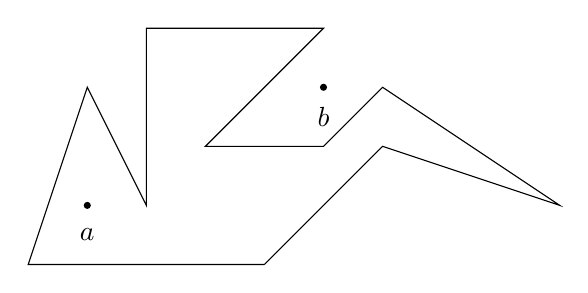
\begin{tikzpicture}[scale=0.75]
%\draw (0,0)--(2,-2)--(3,1)--(5,1)--(2,3)--(1,2)--(-1,2)--(1,4)--(-2,4)--(-2,1)--(-3,3)--(-4,0)--(0,0);
\draw (0,0)--(2,2)--(5,1)--(2,3)--(1,2)--(-1,2)--(1,4)--(-2,4)--(-2,1)--(-3,3)--(-4,0)--(0,0);

\draw[fill] (-3,1) circle [radius=0.05];
\node at (-3,0.5) {$a$};
\draw[fill] (1,3) circle [radius=0.05];
\node at (1,2.5) {$b$};
\end{tikzpicture}
\end{center}

A convenient way to solve the problem is to
send a ray from the point to an arbitrary direction
and calculate the number of times it touches
the boundary of the polygon.
If the number is odd,
the point is inside the polygon,
and if the number is even,
the point is outside the polygon.

\begin{samepage}
For example, we could send the following rays:
\begin{center}
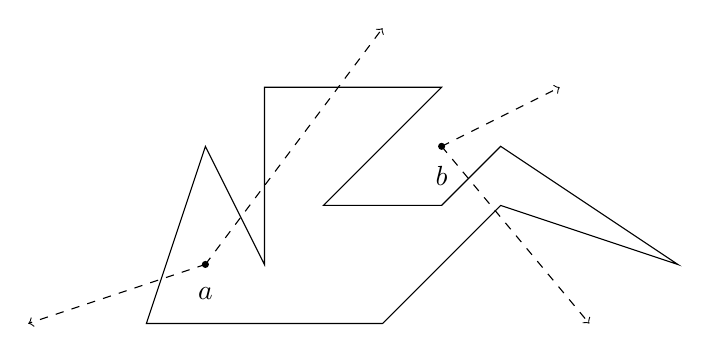
\begin{tikzpicture}[scale=0.75]
\draw (0,0)--(2,2)--(5,1)--(2,3)--(1,2)--(-1,2)--(1,4)--(-2,4)--(-2,1)--(-3,3)--(-4,0)--(0,0);

\draw[fill] (-3,1) circle [radius=0.05];
\node at (-3,0.5) {$a$};
\draw[fill] (1,3) circle [radius=0.05];
\node at (1,2.5) {$b$};

\draw[dashed,->] (-3,1)--(-6,0);
\draw[dashed,->] (-3,1)--(0,5);

\draw[dashed,->] (1,3)--(3.5,0);
\draw[dashed,->] (1,3)--(3,4);
\end{tikzpicture}
\end{center}
\end{samepage}

The rays from $a$ touch 1 and 3 times
the boundary of the polygon,
so $a$ is inside the polygon.
Correspondingly, the rays from $b$
touch 0 and 2 times the boundary of the polygon,
so $b$ is outside the polygon.

\section{Polygon area}

A general formula for calculating the area
of a polygon\footnote{This formula is sometimes called the
\index{shoelace formula} \key{shoelace formula}.} is
\[\frac{1}{2} |\sum_{i=1}^{n-1} (p_i \times p_{i+1})| =
\frac{1}{2} |\sum_{i=1}^{n-1} (x_i y_{i+1} - x_{i+1} y_i)|, \]
where the vertices are
$p_1=(x_1,y_1)$, $p_2=(x_2,y_2)$, $\ldots$, $p_n=(x_n,y_n)$
in such an order that
$p_i$ and $p_{i+1}$ are adjacent vertices on the boundary
of the polygon,
and the first and last vertex is the same, i.e., $p_1=p_n$.

For example, the area of the polygon
\begin{center}
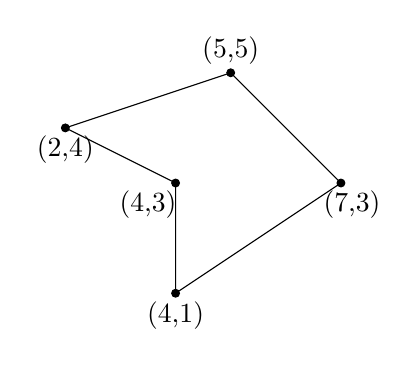
\begin{tikzpicture}[scale=0.7]
\filldraw (4,1.4) circle (2pt);
\filldraw (7,3.4) circle (2pt);
\filldraw (5,5.4) circle (2pt);
\filldraw (2,4.4) circle (2pt);
\filldraw (4,3.4) circle (2pt);
\node (1) at (4,1) {(4,1)};
\node (2) at (7.2,3) {(7,3)};
\node (3) at (5,5.8) {(5,5)};
\node (4) at (2,4) {(2,4)};
\node (5) at (3.5,3) {(4,3)};
\path[draw] (4,1.4) -- (7,3.4) -- (5,5.4) -- (2,4.4) -- (4,3.4) -- (4,1.4);
\end{tikzpicture}
\end{center}
is
\[\frac{|(2\cdot5-5\cdot4)+(5\cdot3-7\cdot5)+(7\cdot1-4\cdot3)+(4\cdot3-4\cdot1)+(4\cdot4-2\cdot3)|}{2} = 17/2.\]

The idea in the formula is to go through trapezoids
whose one side is a side of the polygon,
and another side lies on the horizontal line $y=0$.
For example:
\begin{center}
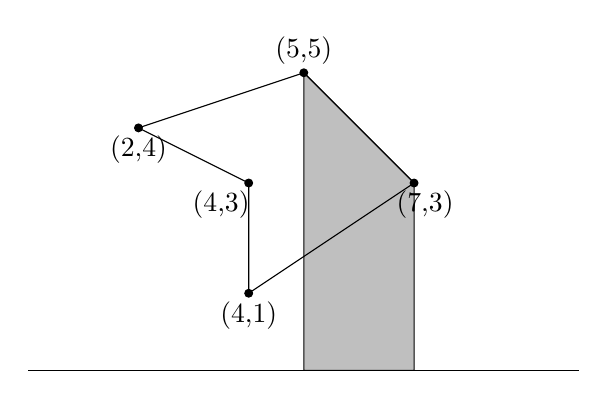
\begin{tikzpicture}[scale=0.7]
\path[draw,fill=lightgray] (5,5.4) -- (7,3.4) -- (7,0) -- (5,0) -- (5,5.4);
\filldraw (4,1.4) circle (2pt);
\filldraw (7,3.4) circle (2pt);
\filldraw (5,5.4) circle (2pt);
\filldraw (2,4.4) circle (2pt);
\filldraw (4,3.4) circle (2pt);
\node (1) at (4,1) {(4,1)};
\node (2) at (7.2,3) {(7,3)};
\node (3) at (5,5.8) {(5,5)};
\node (4) at (2,4) {(2,4)};
\node (5) at (3.5,3) {(4,3)};
\path[draw] (4,1.4) -- (7,3.4) -- (5,5.4) -- (2,4.4) -- (4,3.4) -- (4,1.4);
\draw (0,0) -- (10,0);
\end{tikzpicture}
\end{center}
The area of such a trapezoid is
\[(x_{i+1}-x_{i}) \frac{y_i+y_{i+1}}{2},\]
where the vertices of the polygon are $p_i$ and $p_{i+1}$.
If $x_{i+1}>x_{i}$, the area is positive,
and if $x_{i+1}<x_{i}$, the area is negative.

The area of the polygon is the sum of areas of
all such trapezoids, which yields the formula

\[|\sum_{i=1}^{n-1} (x_{i+1}-x_{i}) \frac{y_i+y_{i+1}}{2}| =
\frac{1}{2} |\sum_{i=1}^{n-1} (x_i y_{i+1} - x_{i+1} y_i)|.\]

Note that the absolute value of the sum is taken,
because the value of the sum may be positive or negative
depending on whether we walk clockwise or counterclockwise
along the boundary of the polygon.

\subsubsection{Pick's theorem}

\index{Pick's theorem}

\key{Pick's theorem} provides another way to calculate
the area of a polygon provided that all vertices 
of the polygon have integer coordinates.
According to Pick's theorem, the area of the polygon is
\[ a + b/2 -1,\]
where $a$ is the number of integer points inside the polygon
and $b$ is the number of integer points on the boundary of the polygon.

For example, the area of the polygon
\begin{center}
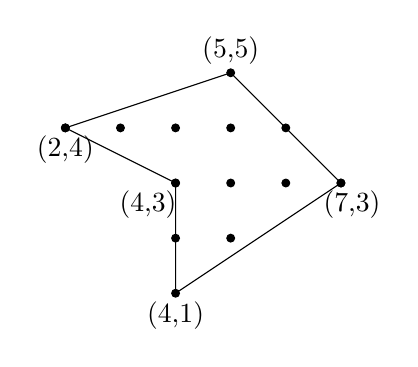
\begin{tikzpicture}[scale=0.7]
\filldraw (4,1.4) circle (2pt);
\filldraw (7,3.4) circle (2pt);
\filldraw (5,5.4) circle (2pt);
\filldraw (2,4.4) circle (2pt);
\filldraw (4,3.4) circle (2pt);
\node (1) at (4,1) {(4,1)};
\node (2) at (7.2,3) {(7,3)};
\node (3) at (5,5.8) {(5,5)};
\node (4) at (2,4) {(2,4)};
\node (5) at (3.5,3) {(4,3)};
\path[draw] (4,1.4) -- (7,3.4) -- (5,5.4) -- (2,4.4) -- (4,3.4) -- (4,1.4);

\filldraw (2,4.4) circle (2pt);
\filldraw (3,4.4) circle (2pt);
\filldraw (4,4.4) circle (2pt);
\filldraw (5,4.4) circle (2pt);
\filldraw (6,4.4) circle (2pt);

\filldraw (4,3.4) circle (2pt);
\filldraw (5,3.4) circle (2pt);
\filldraw (6,3.4) circle (2pt);
\filldraw (7,3.4) circle (2pt);

\filldraw (4,2.4) circle (2pt);
\filldraw (5,2.4) circle (2pt);
\end{tikzpicture}
\end{center}
is $6+7/2-1=17/2$.

\section{Distance functions}

\index{distance function}
\index{Euklidean distance}
\index{Manhattan distance}

A \key{distance function} defines the distance between
two points.
The usual distance function in geometry is the
\key{Euclidean distance} where the distance between
points $(x_1,y_1)$ and $(x_2,y_2)$ is
\[\sqrt{(x_2-x_1)^2+(y_2-y_1)^2}.\]
An alternative distance function is the
\key{Manhattan distance}
where the distance between points
$(x_1,y_1)$ and $(x_2,y_2)$ is
\[|x_1-x_2|+|y_1-y_2|.\]
\begin{samepage}
For example, consider the following picture:
\begin{center}
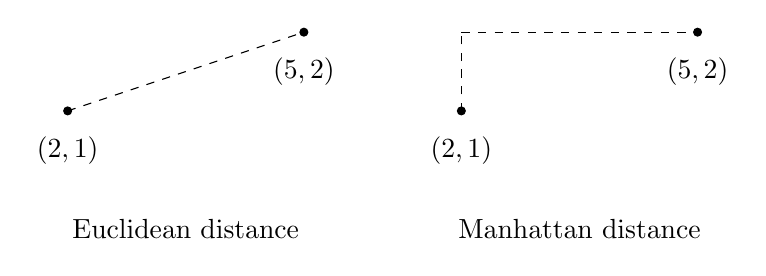
\begin{tikzpicture}

\draw[fill] (2,1) circle [radius=0.05];
\draw[fill] (5,2) circle [radius=0.05];

\node at (2,0.5) {$(2,1)$};
\node at (5,1.5) {$(5,2)$};

\draw[dashed] (2,1) -- (5,2);

\draw[fill] (5+2,1) circle [radius=0.05];
\draw[fill] (5+5,2) circle [radius=0.05];

\node at (5+2,0.5) {$(2,1)$};
\node at (5+5,1.5) {$(5,2)$};

\draw[dashed] (5+2,1) -- (5+2,2);
\draw[dashed] (5+2,2) -- (5+5,2);

\node at (3.5,-0.5) {Euclidean distance};
\node at (5+3.5,-0.5) {Manhattan distance};
\end{tikzpicture}
\end{center}
\end{samepage}
The Euclidean distance between the points is
\[\sqrt{(5-2)^2+(2-1)^2}=\sqrt{10}\]
and the Manhattan distance is
\[|5-2|+|2-1|=4.\]
The following picture shows regions that are within a distance of 1
from the center point, using the Euclidean and Manhattan distances:
\begin{center}
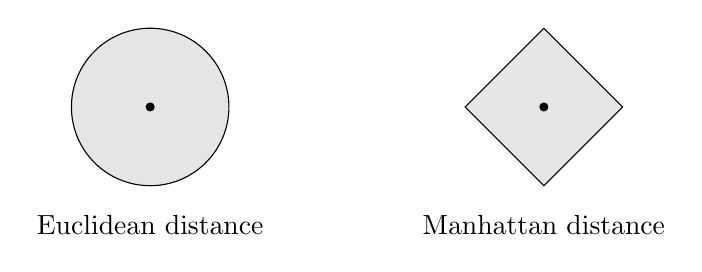
\begin{tikzpicture}

\draw[fill=gray!20] (0,0) circle [radius=1];
\draw[fill] (0,0) circle [radius=0.05];

\node at (0,-1.5) {Euclidean distance};

\draw[fill=gray!20] (5+0,1) -- (5-1,0) -- (5+0,-1) -- (5+1,0) -- (5+0,1);
\draw[fill] (5,0) circle [radius=0.05];
\node at (5,-1.5) {Manhattan distance};
\end{tikzpicture}
\end{center}

\subsubsection{Rotating coordinates}

Some problems are easier to solve if the
Manhattan distance is used instead of the Euclidean distance.
As an example, consider a problem where we are given
$n$ points in the two-dimensional plane
and our task is to calculate the maximum Manhattan
distance between any two points.

For example, consider the following set of points:
\begin{center}
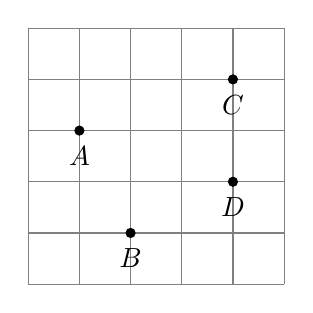
\begin{tikzpicture}[scale=0.65]
\draw[color=gray] (-1,-1) grid (4,4);

\filldraw (0,2) circle (2.5pt);
\filldraw (3,3) circle (2.5pt);
\filldraw (1,0) circle (2.5pt);
\filldraw (3,1) circle (2.5pt);

\node at (0,1.5) {$A$};
\node at (3,2.5) {$C$};
\node at (1,-0.5) {$B$};
\node at (3,0.5) {$D$};
\end{tikzpicture}
\end{center}

The maximum Manhattan distance is 5
between points $B$ and $C$:
\begin{center}
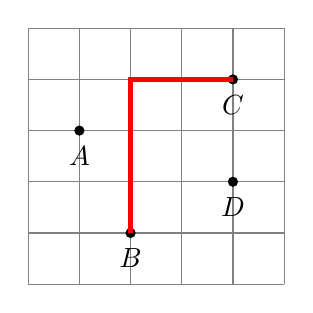
\begin{tikzpicture}[scale=0.65]
\draw[color=gray] (-1,-1) grid (4,4);

\filldraw (0,2) circle (2.5pt);
\filldraw (3,3) circle (2.5pt);
\filldraw (1,0) circle (2.5pt);
\filldraw (3,1) circle (2.5pt);

\node at (0,1.5) {$A$};
\node at (3,2.5) {$C$};
\node at (1,-0.5) {$B$};
\node at (3,0.5) {$D$};

\path[draw=red,thick,line width=2pt] (1,0) -- (1,3) -- (3,3);
\end{tikzpicture}
\end{center}

A useful technique related to Manhattan distances
is to rotate all coordinates 45 degrees so that
a point $(x,y)$ becomes $(x+y,y-x)$.
For example, after rotating the above points,
the result is:

\begin{center}
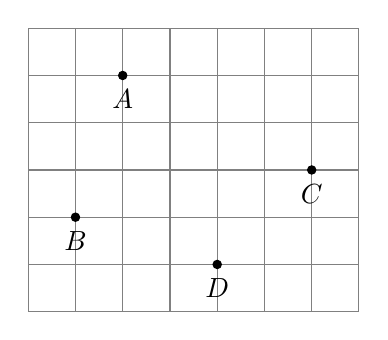
\begin{tikzpicture}[scale=0.6]
\draw[color=gray] (0,-3) grid (7,3);

\filldraw (2,2) circle (2.5pt);
\filldraw (6,0) circle (2.5pt);
\filldraw (1,-1) circle (2.5pt);
\filldraw (4,-2) circle (2.5pt);

\node at (2,1.5) {$A$};
\node at (6,-0.5) {$C$};
\node at (1,-1.5) {$B$};
\node at (4,-2.5) {$D$};
\end{tikzpicture}
\end{center}

And the maximum distance is as follows:
\begin{center}
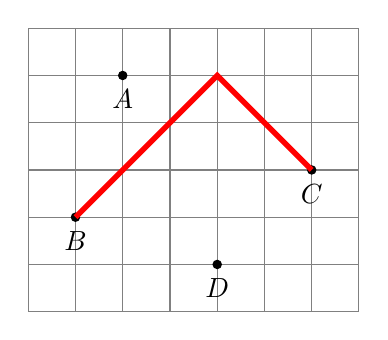
\begin{tikzpicture}[scale=0.6]
\draw[color=gray] (0,-3) grid (7,3);

\filldraw (2,2) circle (2.5pt);
\filldraw (6,0) circle (2.5pt);
\filldraw (1,-1) circle (2.5pt);
\filldraw (4,-2) circle (2.5pt);

\node at (2,1.5) {$A$};
\node at (6,-0.5) {$C$};
\node at (1,-1.5) {$B$};
\node at (4,-2.5) {$D$};

\path[draw=red,thick,line width=2pt] (1,-1) -- (4,2) -- (6,0);
\end{tikzpicture}
\end{center}

Consider two points $p_1=(x_1,y_1)$ and $p_2=(x_1,y_1)$ whose rotated
coordinates are $p'_1=(x'_1,y'_1)$ and $p'_2=(x'_2,y'_2)$.
The Manhattan distance is
\[|x_1-x_2|+|y_1-y_2| = \max(|x'_1-x'_2|,|y'_1-y'_2|)\]

For example, if $p_1=(1,0)$ and $p_2=(3,3)$,
the rotated coordinates are $p'_1=(1,-1)$ and $p'_2=(6,0)$
and the Manhattan distance is
\[|1-3|+|0-3| = \max(|1-6|,|-1-0|) = 5.\]

The rotated coordinates provide a simple way
to operate with Manhattan distances, because we can
consider x and y coordinates separately.
To maximize the Manhattan distance between two points,
we should find two points whose
rotated coordinates maximize the value of
\[\max(|x'_1-x'_2|,|y'_1-y'_2|).\]
This is easy, because either the horizontal or vertical
difference of the rotated coordinates has to be maximum.